%
% Machine Learning Course Homework1
% Only available in ZJU
%
\documentclass[12pt,twoside]{article}

\input{macros}

\usepackage{amsmath}
\usepackage{amssymb}
\usepackage{url}
\usepackage{mdwlist}
\usepackage{graphicx}
\usepackage{clrscode3e}
\newcommand{\isnotequal}{\mathrel{\scalebox{0.8}[1]{!}\hspace*{1pt}\scalebox{0.8}[1]{=}}}
\usepackage{listings}
\usepackage{tikz}
\usetikzlibrary{arrows}
\usetikzlibrary{matrix}
\usetikzlibrary{positioning}
\usetikzlibrary{shapes.geometric}
\usetikzlibrary{shapes.misc}
\usetikzlibrary{trees}

\newcommand{\answer}{
 \par\medskip
 \textbf{Answer:}
}

\newcommand{\collaborators}{ \textbf{Collaborators:}
%%% COLLABORATORS START %%%

\tabT Name: Ge Yuting

\tabT Student ID: 3170103639
%%% COLLABORATORS END %%%
}

\newcommand{\answerIa}{ \answer
%%% PROBLEM 1(a) ANSWER START %%%
\begin{enumerate}
	\item clustering \& unsupervised learning
	\item not learning
	\item classification \& supervised learning
	\item dimensionality reduction
	\item regression \& supervised learning
	\item classification \& supervised learning
	\item clustering \& unsupervised learning
	\item regression \& supervised learning
	\item dimensionality reduction
\end{enumerate}
%%% PROBLEM 1(a) ANSWER END %%%
}

\newcommand{\answerIb}{ \answer
%%% PROBLEM 1(b) ANSWER START %%%
False. The amount of data and parameters depends on many factors, such as the complexity of our problem and learning algorithm. 
%%% PROBLEM 1(b) ANSWER END %%%
}

\newcommand{\answerIIa}{ \answer
%%% PROBLEM 2(a) ANSWER START %%%
\begin{enumerate}
	\item $$P(B_1=1)=\frac{1}{3}$$
	\item $$P(B_2=0|B_1=1)=1$$
	\item $$P(B_1=1|B_2=0)=\frac{P(B_2=0|B_1=1)*P(B_1=1)}{P(B_2=0)}=\frac{1}{3}$$
	\item I will choose the only left box $B_3$, because:
	$$P(B_3=1|B_2=0)=\frac{P(B_2=0|B_3=1)*P(B_3=1)}{P(B_2=0)}=\frac{2}{3}$$
	$$P(B_3=1|B_2=0)>P(B_1=1|B_2=0)$$
\end{enumerate}
%%% PROBLEM 2(a) ANSWER END %%%
}
\newcommand{\answerIIb}{ \answer
%%% PROBLEM 2(b) ANSWER START %%%
\begin{enumerate}
	\item 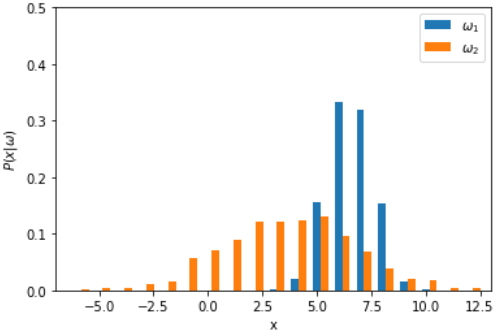
\includegraphics[scale=0.7]{1.png} 
	\item 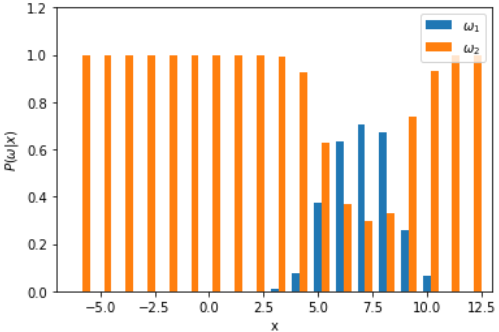
\includegraphics[scale=0.7]{2.png} 
	\item minimal risk: 1.0\\
\end{enumerate}
%%% PROBLEM 2(b) ANSWER END %%%
}



\newcommand{\answerIIIa}{ \answer 
%%% PROBLEM 3(a) ANSWER START %%%
$$p(y=1|\textbf{x})=\frac{p(\textbf{x}|y=1)*p(y=1)}{\sum_{n=0}^1p(\textbf{x}|y=n)*p(y=n)}=\frac{p(\textbf{x}|y=1)*p(y=1)}{p(\textbf{x}|y=0)*p(y=0)+p(\textbf{x}|y=1)*p(y=1)}$$
$$=\frac{\frac{1}{2\pi\sqrt{|\Sigma_1|}}\exp[-\frac{1}{2}(\textbf{x}-\mu_1)^T{\Sigma_1}^{-1}(\textbf{x}-\mu_1)]}{{\frac{1}{2\pi\sqrt{|\Sigma_0|}}\exp[-\frac{1}{2}(\textbf{x}-\mu_0)^T{\Sigma_0}^{-1}(\textbf{x}-\mu_0)]}+{\frac{1}{2\pi\sqrt{|\Sigma_1|}}\exp[-\frac{1}{2}(\textbf{x}-\mu_1)^T{\Sigma_1}^{-1}(\textbf{x}-\mu_1)]}}$$
$$=\frac{exp[-\frac{1}{2}((x_1-1)^2+(x_2-1)^2)]}{{exp[-\frac{1}{2}({x_1}^2+{x_2}^2)]}+{exp[-\frac{1}{2}((x_1-1)^2+(x_2-1)^2)]}}$$
$$=\frac{1}{e^{x_1+x_2-1}+1}$$
\\decision boundary: 
$$\because{p(y=1|\textbf{x})=p(y=0|\textbf{x})}$$
$$\therefore{1-x_1-x_2=0} $$
%%% PROBLEM 3(a) ANSWER END %%%

}
\newcommand{\answerIIIb}{ \answer
	%%% PROBLEM 3(b) ANSWER START %%%
in \textit{gaussian\_pos\_prob.py}
	%%% PROBLEM 3(b) ANSWER END %%%
}
\newcommand{\answerIIIc}{ \answer
%%% PROBLEM 3(c) ANSWER START %%%
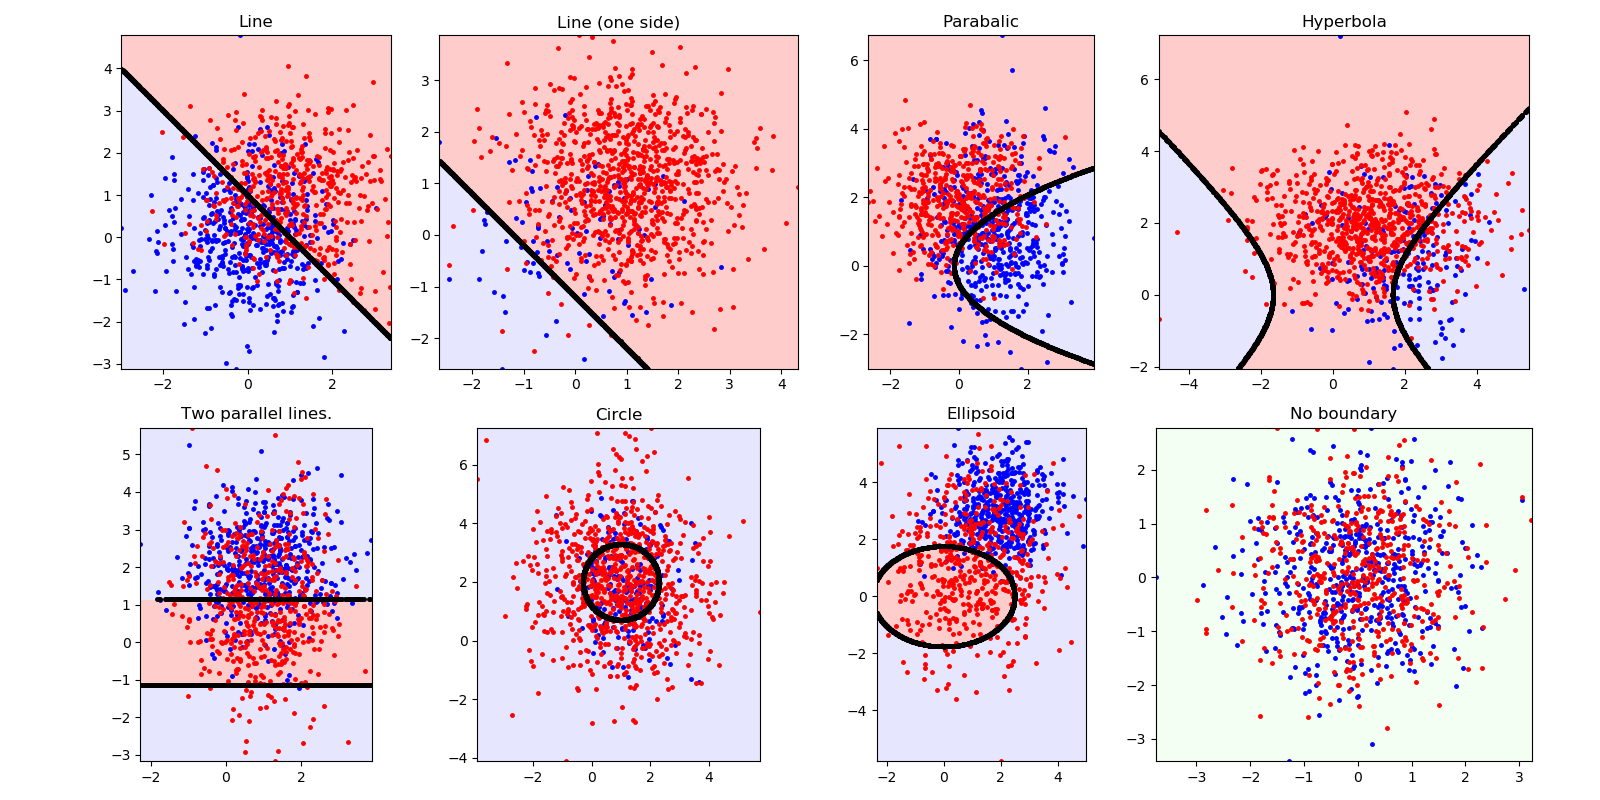
\includegraphics[scale=0.3]{hw1_gaussian_discriminant.png}
%%% PROBLEM 3(c) ANSWER END %%%
}

\newcommand{\answerIIId}{ \answer
%%% PROBLEM 3(d) ANSWER START %%%


%%% PROBLEM 3(d) ANSWER END %%%
}
\newcommand{\answerIIIIa}{ \answer
%%% PROBLEM 4(a) ANSWER START %%%

%%% PROBLEM 4(a) ANSWER END %%%
}
\newcommand{\answerIIIIb}{ \answer
%%% PROBLEM 4(b) ANSWER START %%%

%%% PROBLEM 4(b) ANSWER END %%%
}
\newcommand{\answerIIIIc}{ \answer
%%% PROBLEM 4(c) ANSWER START %%%

%%% PROBLEM 4(c) ANSWER END %%%
}
\newcommand{\answerIIIId}{ \answer
%%% PROBLEM 4(d) ANSWER START %%%

%%% PROBLEM 4(d) ANSWER END %%%
}
\newcommand{\answerIIIIe}{ \answer
%%% PROBLEM 4(e) ANSWER START %%%

%% PROBLEM 4(e) ANSWER END %%%
}

\setlength{\oddsidemargin}{0pt}
\setlength{\evensidemargin}{0pt}
\setlength{\textwidth}{6.5in}
\setlength{\topmargin}{0in}
\setlength{\textheight}{8.5in}

% Fill these in!
\newcommand{\theproblemsetnum}{1}
\newcommand{\releasedate}{April 27, 2020}
\newcommand{\partaduedate}{May 14, 2019}
\newcommand{\tabUnit}{3ex}
\newcommand{\tabT}{\hspace*{\tabUnit}}

\begin{document}

\handout{Homework \theproblemsetnum}{\releasedate}



\collaborators
% Please download the .zip archive for this problem set, and refer to the
% hw1.pdf file for instructions on preparing your solutions.
%


\medskip

\hrulefill

\begin{problems}

\problem \textbf{Machine Learning Problems}
\begin{problemparts}
\problempart Choose proper word(s) from
\answerIa


\problempart True or False: “To fully utilizing available data resource, we should use all the data we
have to train our learning model and choose the parameters that maximize performance
on the whole dataset.” Justify your answer.
\answerIb

\end{problemparts}
\newpage

\problem \textbf{Bayes Decision Rule}
\begin{problemparts}
\problempart
Suppose you are given a chance to win bonus grade points:


\answerIIa

\problempart Now let us use bayes decision theorem to make a two-class classifier $\cdots$.

\answerIIb


\end{problemparts}
\newpage
\problem \textbf{Gaussian Discriminant Analysis and MLE}

Given a dataset consisting of m samples. We assume these samples are independently generated by one of two Gaussian distributions$\cdots$
\begin {problemparts}
\problempart What is the decision boundary?

\answerIIIa

\problempart An extension of the above model is to classify K classes by fitting a Gaussian distribution for each class$\cdots$
\answerIIIb

\problempart  Now let us do some field work – playing with the above 2-class Gaussian discriminant model.
\answerIIIc

\problempart What is the maximum likelihood estimation of $\phi, \mu_0$ and $\mu_1$?
\answerIIId 

\end{problemparts}

\newpage

\problem  \textbf{Text Classification with Naive Bayes}

\begin{problemparts}
\problempart  List the top 10 words.

\answerIIIIa

\problempart What is the accuracy of your spam filter on the testing set?
\answerIIIIb

\problempart True or False: a model with 99\% accuracy is always a good model. Why?
\answerIIIIc

\problempart Compute the precision and recall of your learnt model.
\answerIIIId 

\problempart For a spam filter, which one do you think is more important, precision or recall? What about a classifier to identify drugs and bombs at airport? Justify your answer.
\answerIIIIe 

\end{problemparts}

\end{problems}
\end{document}
